\section{GPSBench}
\label{sec:gpsbench}

GPSBench comprises \textbf{57,800 samples} across 17 tasks, organized into two tracks: the \textit{Pure GPS Track} (9 tasks) testing coordinate operations and the \textit{Applied Track} (8 tasks) requiring geographic knowledge. Each task contains 3,400 samples split into train (60\%), dev (10\%), and test (30\%).

%==============================================================================
\subsection{Benchmark Design}
\label{sec:benchmark}
%==============================================================================

GPSBench evaluates \textbf{intrinsic spatial knowledge}---not tool-use ability. This distinction matters because: (1) tool-augmented evaluations conflate model knowledge with API availability, revealing nothing about internal representations; (2) existing benchmarks like GeoBenchX \citep{krechetova2025geobenchx} evaluate workflow orchestration, while GPSBench tests the underlying knowledge such tools would provide; (3) performance gaps across regions expose training biases that tool augmentation would mask; and (4) many deployments---latency-sensitive, offline, or privacy-restricted---preclude API calls. Our protocol (Section~\ref{sec:experiments}) enforces this: models respond from parametric knowledge alone.

Following the landmark-route-survey framework from spatial cognition research \citep{siegel1975development}, we organize tasks by the type of spatial representation required:

\begin{itemize}[leftmargin=*, itemsep=2pt]
    \item \textbf{Landmark (L):} Recognizing individual locations from coordinates---the most basic spatial representation, requiring no metric relations between places.
    \item \textbf{Route (R):} Sequential, procedural understanding of paths connecting locations---egocentric representations learned through navigation.
    \item \textbf{Survey (S):} Allocentric, map-like representations with metric information enabling global spatial reasoning across locations.
    \item \textbf{Geometric (G):} Pure mathematical operations on coordinates requiring no geographic knowledge---a control condition isolating computational from world-knowledge capabilities.
\end{itemize}

Table~\ref{tab:task_summary} summarizes all tasks with their spatial knowledge type.

\begin{table*}[t]
\centering
\caption{Summary of GPSBench tasks organized by spatial knowledge type following the landmark-route-survey framework \citep{siegel1975development}. Types: \textbf{L}=Landmark, \textbf{R}=Route, \textbf{S}=Survey, \textbf{G}=Geometric (no world knowledge).}
\label{tab:task_summary}
\small
\begin{tabular}{@{}llp{7.5cm}cc@{}}
\toprule
\textbf{Track} & \textbf{Task} & \textbf{Sample} & \textbf{Type} & \textbf{N} \\
\midrule
\multirow{9}{*}{\rotatebox[origin=c]{90}{Pure GPS}}
& Format Conversion & Convert 32°3'9.0"S, 115°53'16.2"E to decimal $\rightarrow$ \textit{-32.0525, 115.8878} & G & 3,400 \\
& Coord. Transform & Transform (19.37, 95.22) to UTM $\rightarrow$ \textit{Zone 46N, 732668E, 2143080N} & G & 3,400 \\
& Distance Calc. & Distance from (-2.13, -47.56) to (-22.63, -47.05)? $\rightarrow$ \textit{2,280 km} & G, S & 3,400 \\
& Bearing Comp. & Bearing from (49.28, -123.13) to (5.89, 5.68)? $\rightarrow$ \textit{55.2° (NE)} & G, S & 3,400 \\
& Interpolation & 50\% along (29.93, 117.95) to (-6.99, 106.55)? $\rightarrow$ \textit{(11.53, 111.86)} & G, R & 3,400 \\
& Area \& Perimeter & Area of polygon [(-2.85, 33.08), (21.15, 72.96), (29.35, 105.89)]? $\rightarrow$ \textit{30,829 km²} & G, S & 3,400 \\
& Bounding Box & Center of [(-2.85, 33.08), (21.15, 72.96), (53.60, 24.75), ...]? $\rightarrow$ \textit{(7.82, 52.08)} & G, S & 3,400 \\
& Route Geometry & Simplify 12-point path ($\epsilon$=1.3km) $\rightarrow$ \textit{keep [0,1,4,5,6,7,11]} & G, R & 3,400 \\
& Relative Position & Direction from (40.25, -8.39) to (0.06, 34.29)? $\rightarrow$ \textit{West} & G, S & 3,400 \\
\midrule
\multirow{8}{*}{\rotatebox[origin=c]{90}{Applied}}
& Place Association & City at (41.12, -8.65)? $\rightarrow$ \textit{Canidelo, Portugal} & L & 3,400 \\
& Name Disambig. & 4 cities named ``Nawābganj''. Which at (26.93, 81.20)? $\rightarrow$ \textit{B (India)} & L & 3,400 \\
& Relative Position & Mikkeli to Sosnovka? $\rightarrow$ \textit{South} & L, S & 3,400 \\
& Proximity & Closest to Titirangi: Elsdorf, Itatim, Murray, Cianjur? $\rightarrow$ \textit{Murray} & L, S & 3,400 \\
& Route Analysis & Canberra on Gröbenzell→Dois Irmãos? $\rightarrow$ \textit{No} & L, R & 3,400 \\
& Spatial Patterns & Outlier: Mornington, Ringwood, Caroline Springs, Ballajura, Sonneberg? $\rightarrow$ \textit{Sonneberg} & L, S & 3,400 \\
& Boundary Analysis & Group by continent: Corroios, Wimbledon, Toms River, Santa Ana $\rightarrow$ \textit{\{EU: 2, NA: 2\}} & L, S & 3,400 \\
& Terrain Class. & Terrain at (-27.47, 153.03)? $\rightarrow$ \textit{Coastal} & L & 3,400 \\
\midrule
\multicolumn{4}{r}{\textbf{Total: Train 34,680 / Dev 5,780 / Test 17,340}} & \textbf{57,800} \\
\bottomrule
\end{tabular}
\end{table*}

%==============================================================================
\subsection{Data Generation}
%==============================================================================

\paragraph{Data Source.}
We leverage the \textbf{GeoNames database}\footnote{\url{https://www.geonames.org/}} (\texttt{cities15000.txt}), containing 32,709 cities with populations exceeding 15,000. Each entry provides WGS84 coordinates, city/country identifiers, population statistics, and alternate name spellings, ensuring global coverage across 200+ countries. Figure~\ref{fig:world_map} shows the geographic distribution of 18,196 unique locations used in GPSBench.

\begin{figure}[htbp]
\centering
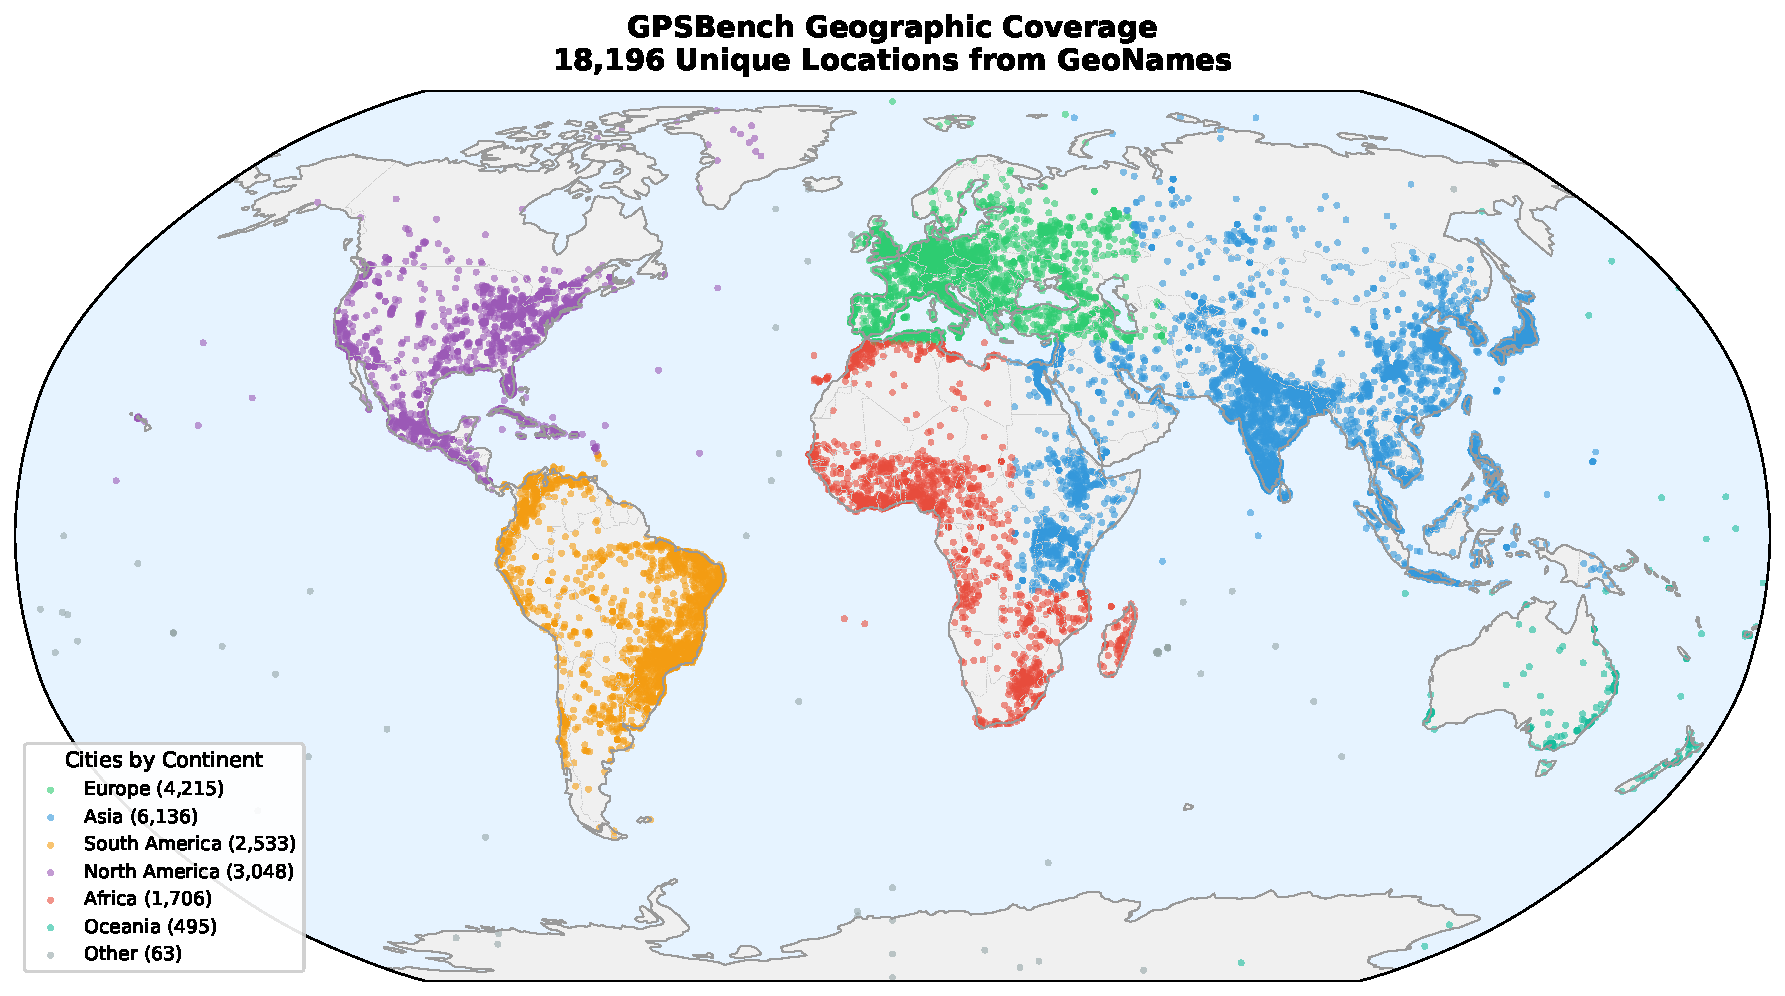
\includegraphics[width=\columnwidth]{figures/world_map_coverage.pdf}
\caption{Geographic coverage of GPSBench. 18,196 unique locations from GeoNames span all continents: Asia (33.7\%), Europe (23.2\%), North America (16.8\%), South America (13.9\%), Africa (9.4\%), and Oceania (2.7\%).}
\label{fig:world_map}
\end{figure}

\paragraph{Sample Generation Pipeline.}
Each task follows a structured generation pipeline: (1) \textit{city selection} using task-appropriate sampling strategy, (2) \textit{input construction} by applying task-specific transformations, and (3) \textit{ground truth computation} using geodetic formulas or database lookups. For Pure GPS tasks, we select cities globally, extract coordinates, and compute answers programmatically (e.g., Haversine distance, spherical bearing). For Applied tasks, we select cities based on task constraints (e.g., same-continent pairs for Relative Position, cities with duplicate names for Name Disambiguation), then test whether models can recover geographic facts from coordinates alone. All generation uses a fixed random seed for reproducibility. See Appendix~\ref{app:data_generation} for per-task generation details.

\paragraph{Geographic Diversity.}
Raw GeoNames data is skewed toward Asia (36.6\%) and Europe (24.0\%), with Oceania underrepresented (1.2\%). We address this through \textit{stratified continent-balanced sampling}: target quotas rebalance toward underrepresented regions (Africa: 20\%, Oceania: 5\%) while enforcing 100~km minimum separation between selected cities to prevent geographic clustering. For tasks requiring spatial relationships (e.g., Polygon Area, Spatial Patterns), we use \textit{regional sampling} that constrains selections to same-continent cities within 50--2,000~km, creating realistic polygon sizes comparable to countries or states.

\paragraph{Difficulty Control.}
We control difficulty through three mechanisms: (1) \textit{Population tiers} for Place Association (easy: $>$500K, medium: 100--500K, hard: $<$100K); (2) \textit{Distance ranges} for Applied Relative Position (200--500~km is hardest, 2,000--3,000~km is easier); and (3) \textit{Coordinate noise} for Place Association and Name Disambiguation (Gaussian noise $\sigma \in \{0, 10, 50, 100, 500, 1000\}$~m), simulating conditions from precise GPS ($\pm$10~m) to coarse positioning ($\pm$1~km). Noise also prevents shortcut solutions via exact coordinate memorization.

\paragraph{Ground Truth Computation.}
For \textit{geometric tasks} (Pure GPS Track), we apply standard geodetic formulas on the WGS84 ellipsoid approximated as a sphere ($R = 6371$~km): Haversine for distance, forward azimuth for bearing, spherical linear interpolation (slerp) for intermediate points, and L'Huilier's theorem for spherical polygon area. Coordinate transformations use Transverse Mercator (UTM) and Web Mercator (EPSG:3857). For \textit{knowledge-based tasks} (Applied Track), ground truth derives from GeoNames metadata: city names for Place Association, country/continent codes for Boundary Analysis, and computed Haversine distances for Proximity and Spatial Patterns. All answers are deterministic and programmatically verifiable. Full formulas are provided in Appendix~\ref{app:ground_truth_formulas}.

\paragraph{Quality Assurance.}
We validate all 57,800 samples through automated verification: coordinate range checks (latitude $\in [-90°, 90°]$, longitude $\in [-180°, 180°]$), bidirectional conversion verification for Format Conversion, distance calculations cross-checked against the Vincenty formula, and statistical verification that noise distributions match theoretical Rayleigh distributions. Train/dev/test splits (60\%/10\%/30\%) are verified to have zero sample overlap. See Appendix~\ref{app:quality_assurance} for validation details.

Full task prompts are provided in Appendix~\ref{app:task_prompts}.

